\chapter{Einleitung}
\section{Ausgangssituation}
Die HTL Leonding ist ausgestattet mit modernen Multimedia Systemen wie einer Videowall, einem riesigem Touchscreen Tv und mehreren Bildschirmen. Diese Bildschirme werden nicht sehr effektiv genutzt.

\section{Problemstellung}
Momentan wird ein großer Aufwand betrieben, um eine einfache Slideshow von Bildern auf einem Bildschirm anzuzeigen. Da nur ein Video-Format unterstützt wird müssen die Fotos manuell in ein Video verarbeitet werden und dann auf den Bildschirm über einen DVD-Player abgespielt werden. Des Weiteren können keine dynamischen Daten angezeigt werden. Dieser Prozess ist sehr langwierig und ist in der Praxis viel zu aufwendig.

\begin{figure}[h]
\centering
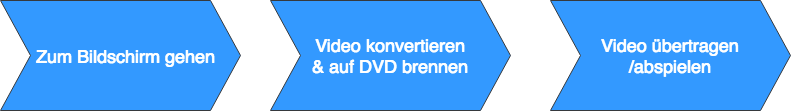
\includegraphics[width=1\textwidth]{images/01_Introduction/WayToDisplay.png}
\caption{Prozess des Anzeigens}
\label{img:processofshow}
\end{figure}

\section{Aufgabenstellung}
Der Aufwand für das erstellen von Slideshows, Informations Elementen soll vermindert werden. Mehrere Datentypen sollen unterstützt werden. Dabei soll auch das Präsentieren von Informatik Projekten erleichtert werden.

\section{Ziele}
Ziel ist es, dass aktuelle Nachrichten oder Informationen den Schülern und Schülerinnen der HTL Leonding näher gebracht werden. Diese Nachrichten können verschiedenster Natur sein zum Beispiel Ankündigungen, Warnung oder sonstige hilfreiche Informationen. Des weiteren soll es der HTL Leonding leichter fallen Informatik Projekte zu präsentieren die 
